\scanpage{20}
\deleted{b) celui qui correspond au plan $(x,y$}

\unsure{Plan Tangent|Plan tangent} : $C$ le long de $D_{\zeta}$

Son équation est (utilisant la matrice
adjointe \deleted{$\unsure{x,y,z}$} $\Delta$) :
\[
Ax+By+Cz=0
\]
\[
\deleted{2x-\alpha y=}
\]
où $A,B,C$ sont donnés par $\Delta\cdot(1,\zeta,0)$ i.e.
\[
\begin{aligned}
 A&=2-\alpha\zeta\deleted{\unsure{0}}, & B&=-\unsure{\zeta}\alpha+2\zeta, & C&=-(1+\zeta)\\
 &=1-\zeta^2\deleted{=\unsure{\zeta(\zeta'-\zeta)}}&&=\zeta-\zeta^{-1}=-\zeta^{-1}(1-\zeta^2)\\
 &=(1-\zeta)(1+\zeta)&&=-\zeta^{-1}(1-\zeta)(1+\zeta)
\end{aligned}
\]
On peut (comme $1+\zeta$ \deleted{\unsure{$=2$}} inv. i.e. $\zeta=-1$ fibre par
fibre i.e. $\alpha\ne-2$ fibre par fibre, par hyp.) \unsure{simplifier|diviser}
par $(1+\zeta)$, on trouve l'équation
\[
H_\zeta:\quad\left\{\begin{aligned}
 (1-\zeta)x-\zeta^{-1}(1-\zeta)y-z&=0\qquad\text{i.e.}\\
 z&=(1-\zeta)(x-\zeta^{-1}y)
\end{aligned}\right.
\]
\diagram{\begin{tikzcd}[ampersand replacement=\&,column sep=small,row sep=small]
D_\zeta \& {\subset H_\zeta} \& {\subset E}\\
\& V\arrow[u,"\unsure{\sim|\simeq}"'] \&
\end{tikzcd}}

Ainsi $C$ s'identifie à la \inserted{clôture projective de} \unsure{l'espace|espace} affine
associé à l'extension de $E/H_\zeta$ par $H_\zeta/D_\zeta\simeq V/D_\zeta\simeq$

Comme l'axe des $z$ \inserted{$(\underline{O}_S e_3)$} est un supplémentaire,
\unsure{icette|ledit} \inserted{espace affine est} \deleted{un} \uline{vectoriel}, isomorphe au fibré
vectoriel cov. associé :
\[
{\underbrace{(E/H_\zeta)}_{\underline{O}_S\cdot e_3}}^{\otimes-1}\otimes
\underbrace{H_\zeta/D_\zeta}_{\simeq\underline{O}_S e_1}
\]

\figure{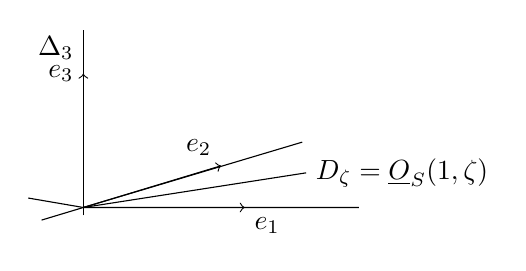
\begin{tikzpicture}[x=1cm,y=1cm]
\draw (-.70,.12)--(0,0)--(3.5,0);
\draw[->] (0,0)--(2.05,0) node[below right] {$e_1$};
\draw (0,-.10)--(0,2.25);
\draw[->] (0,0)--(0,1.7) node[left] {$e_3$};
\node[left] at (0,2.02) {$\unsure{\Delta_3}$};
\draw (-.53,-.16)--(0,0)--(2.78,.83);
\draw[->] (0,0)--(1.75,.53) node[above left] {$e_2$};
\draw (0,0)--(2.83,.44) node[right] {$D_\zeta=\underline{O}_S(1,\zeta)$};
\end{tikzpicture}}

% archive sheet number: 19

